% Fiche de synthèse : le mouvement rectiligne (5e physique, UAA5) -- recto-verso
\documentclass[10pt,a4paper]{article}
\usepackage[T1]{fontenc}
\usepackage[utf8]{inputenc}
\usepackage[scaled]{helvet}
\renewcommand{\familydefault}{\sfdefault}
\usepackage[helvet]{sfmath}
\usepackage{amsmath,amssymb}
\usepackage[margin=1.5cm,top=1.3cm,bottom=1.6cm]{geometry}
\usepackage{tikz}
\usetikzlibrary{arrows.meta,patterns,calc}
\usepackage[most]{tcolorbox}
\usepackage{tabularx,array}
\usepackage{enumitem}
\usepackage{fancyhdr}

\definecolor{marine}{HTML}{1F2A44}
\definecolor{bleu}{HTML}{2A4F86}
\definecolor{fond}{HTML}{F1F4FA}
\definecolor{gris}{HTML}{6B7280}

\pagestyle{fancy}\fancyhf{}
\renewcommand{\headrulewidth}{0pt}
\fancyfoot[R]{\scriptsize\color{gris}Réalisé avec l'aide de l'IA (AIA)}
\setlength{\parindent}{0pt}

% ---------- bandeau de page
\newcommand{\bandeau}[2]{%
\begin{tcolorbox}[enhanced,colback=marine,colframe=marine,arc=3mm,left=4mm,right=4mm,top=1.5mm,bottom=1.5mm]
\color{white}{\Large\bfseries #1}\hfill{\small 5\textsuperscript{e} Physique $\cdot$ UAA5 $\cdot$ fiche de synthèse (#2)}
\end{tcolorbox}\vspace{2mm}}

% ---------- encadré avec onglet
\newtcolorbox{bloc}[2][]{enhanced,breakable=false,colback=white,colframe=bleu,boxrule=0.8pt,arc=3mm,
  attach boxed title to top left={xshift=4mm,yshift=-3mm},
  boxed title style={colback=bleu,colframe=bleu,arc=2mm},
  fonttitle=\bfseries\small\color{white},title={#2},top=4mm,left=2mm,right=2mm,bottom=2mm,#1}

\newcommand{\formule}[1]{\tcbox[on line,colback=fond,colframe=bleu,boxrule=0.5pt,arc=0pt,left=2mm,right=2mm,top=1mm,bottom=1mm]{#1}}

% ---------- mini-graphiques
\tikzset{mg/.style={x=1cm,y=1cm},courbe/.style={bleu,line width=0.9pt},surax/.style={bleu,line width=1.8pt}}
% #1 : nom de l'axe vertical ; #2 : hauteur de l'axe t (0 = en bas) ; #3 : tracé
\newcommand{\mini}[3]{%
\begin{tikzpicture}[mg,scale=1.1,baseline=(current bounding box.center)]
\draw[-{Stealth[length=1.6mm]}] (0,0)--(0,1.25) node[above,inner sep=1pt]{\scriptsize$#1$};
\draw[-{Stealth[length=1.6mm]}] (0,#2)--(1.9,#2) node[below,inner sep=1pt]{\scriptsize$t$};
#3
\end{tikzpicture}}

\begin{document}
%==================================================================== RECTO
\bandeau{Le mouvement rectiligne}{recto}

\begin{bloc}{Décrire un mouvement rectiligne}
\begin{minipage}[t]{0.55\linewidth}
La \textbf{trajectoire est une droite} : on place un axe $x$ le long de cette droite, avec une \textbf{origine O} et un \textbf{sens positif}. Un seul nombre (une composante, avec son signe) suffit pour décrire chaque grandeur vectorielle.

\smallskip
• \textbf{position} $x$ (m) : coordonnée sur l'axe\\
• \textbf{déplacement} $\varDelta x = x_2 - x_1$ (m)\\
• \textbf{durée} $\varDelta t = t_2 - t_1$ (s)\\
• $v > 0$ : sens de l'axe \quad $v < 0$ : sens opposé
\end{minipage}\hfill
\begin{minipage}[t]{0.42\linewidth}
\vspace{4mm}\centering
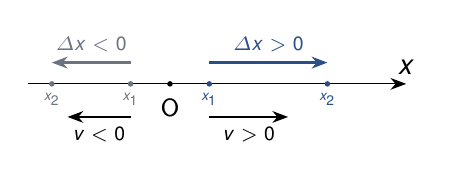
\begin{tikzpicture}[x=1cm,y=1cm]
\draw[-{Stealth[length=2mm]}] (-1.8,0)--(3,0) node[above]{$x$};
\fill (0,0) circle(1pt) node[below=2pt]{\small O};
\foreach \p/\l in {-1.5/x_2,-0.5/x_1}{\fill[gris] (\p,0) circle(1pt) node[below,gris]{\tiny$\l$};}
\foreach \p/\l in {0.5/x_1,2/x_2}{\fill[bleu] (\p,0) circle(1pt) node[below,bleu]{\tiny$\l$};}
\draw[gris,-{Stealth[length=2mm]},line width=1pt] (-0.5,0.27)--(-1.5,0.27) node[midway,above,gris]{\scriptsize$\varDelta x<0$};
\draw[bleu,-{Stealth[length=2mm]},line width=1pt] (0.5,0.27)--(2,0.27) node[midway,above,bleu]{\scriptsize$\varDelta x>0$};
\draw[-{Stealth[length=2mm]}] (-0.5,-0.42)--(-1.3,-0.42) node[midway,below]{\scriptsize$v<0$};
\draw[-{Stealth[length=2mm]}] (0.5,-0.42)--(1.5,-0.42) node[midway,below]{\scriptsize$v>0$};
\end{tikzpicture}
\end{minipage}

\medskip
\centering
\formule{$v_{moy}=\dfrac{\varDelta x}{\varDelta t}$}\quad
\formule{$a_{moy}=\dfrac{\varDelta v}{\varDelta t}$}\quad
\formule{m/s $\xrightarrow{\ \times 3{,}6\ }$ km/h}\quad
\formule{unités : m, s, m/s, m/s$^2$}
\end{bloc}

\vspace{2mm}
\begin{bloc}{Reconnaître le mouvement sur chaque graphique}
\centering
\renewcommand{\arraystretch}{1.15}
\begin{tabular}{@{}m{3cm}ccc@{}}
 & \textbf{position} $x(t)$ & \textbf{vitesse} $v(t)$ & \textbf{accélération} $a(t)$\\[1mm]
\textbf{À l'arrêt}\newline{\scriptsize $v=0$, $a=0$} &
 \mini{x}{0}{\draw[courbe] (0,0.75)--(1.6,0.75);} &
 \mini{v}{0.55}{\draw[surax] (0,0.55)--(1.6,0.55);} &
 \mini{a}{0.55}{\draw[surax] (0,0.55)--(1.6,0.55);}\\
\textbf{MRU}\newline{\scriptsize $v>0$ constante\newline $a=0$} &
 \mini{x}{0}{\draw[courbe] (0,0.15)--(1.6,1.0);} &
 \mini{v}{0.55}{\draw[courbe] (0,0.95)--(1.6,0.95);} &
 \mini{a}{0.55}{\draw[surax] (0,0.55)--(1.6,0.55);}\\
\textbf{MRU}\newline{\scriptsize $v<0$ constante\newline $a=0$} &
 \mini{x}{0}{\draw[courbe] (0,1.0)--(1.6,0.08);} &
 \mini{v}{0.55}{\draw[courbe] (0,0.15)--(1.6,0.15);} &
 \mini{a}{0.55}{\draw[surax] (0,0.55)--(1.6,0.55);}\\
\textbf{MRUA}\newline{\scriptsize $a>0$, $v>0$\newline accélère} &
 \mini{x}{0}{\draw[courbe,domain=0:1.6,samples=30] plot(\x,{0.1+0.12*\x+0.3*\x*\x});} &
 \mini{v}{0}{\draw[courbe] (0,0.25)--(1.6,1.0);} &
 \mini{a}{0.4}{\draw[courbe] (0,0.85)--(1.6,0.85);}\\
\textbf{MRUA}\newline{\scriptsize $a<0$, $v>0$\newline décélère} &
 \mini{x}{0}{\draw[courbe,domain=0:1.6,samples=30] plot(\x,{0.05+1.2*\x-0.37*\x*\x});} &
 \mini{v}{0}{\draw[courbe] (0,1.0)--(1.6,0.12);} &
 \mini{a}{0.75}{\draw[courbe] (0,0.3)--(1.6,0.3);}
\end{tabular}
\end{bloc}

\vspace{2mm}
\begin{minipage}[t]{0.485\linewidth}
\begin{bloc}[height=3.3cm]{MRU : vitesse constante}
$a=0$ \qquad $v=$ constante

\smallskip\centering
\formule{$x(t)=x_0+v\,(t-t_0)$}
\end{bloc}
\end{minipage}\hfill
\begin{minipage}[t]{0.485\linewidth}
\begin{bloc}[height=3.3cm]{MRUA : accélération constante}
$a=$ constante $\neq 0$

\smallskip\centering
\formule{$v(t)=v_0+a\,\varDelta t$}

\smallskip
\formule{$x(t)=x_0+v_0\,\varDelta t+\frac12\,a\,\varDelta t^2$}
\end{bloc}
\end{minipage}

\newpage
%==================================================================== VERSO
\bandeau{Lire un graphique et résoudre un problème}{verso}

\begin{bloc}{Pente et aire : ce que disent les graphiques}
\begin{minipage}[t]{0.25\linewidth}\centering
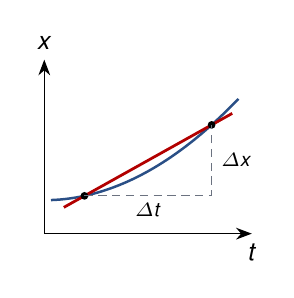
\begin{tikzpicture}[x=0.85cm,y=0.85cm]
\draw[-{Stealth[length=2mm]}] (0,0)--(0,2.6) node[above]{\small$x$};
\draw[-{Stealth[length=2mm]}] (0,0)--(3.1,0) node[below]{\small$t$};
\draw[courbe,domain=0.1:2.9,samples=40] plot(\x,{0.5+0.18*\x*\x});
\coordinate (A) at (0.6,{0.5+0.18*0.36}); \coordinate (B) at (2.5,{0.5+0.18*6.25});
\draw[red!70!black,line width=1pt,shorten <=-3mm,shorten >=-3mm] (A)--(B);
\fill (A) circle(1.4pt) (B) circle(1.4pt);
\draw[densely dashed,gris] (A)--(B|-A) node[midway,below=-1pt,black]{\scriptsize$\varDelta t$}--(B) node[midway,right,black]{\scriptsize$\varDelta x$};
\end{tikzpicture}

\small\textbf{corde} entre deux points :\\ sa pente donne $v_{moy}=\dfrac{\varDelta x}{\varDelta t}$
\end{minipage}\hfill
\begin{minipage}[t]{0.25\linewidth}\centering
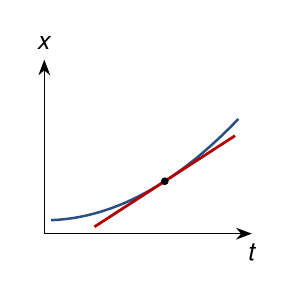
\begin{tikzpicture}[x=0.85cm,y=0.85cm]
\draw[-{Stealth[length=2mm]}] (0,0)--(0,2.6) node[above]{\small$x$};
\draw[-{Stealth[length=2mm]}] (0,0)--(3.1,0) node[below]{\small$t$};
\draw[courbe,domain=0.1:2.9,samples=40] plot(\x,{0.2+0.18*\x*\x});
% tangente en t = 1,8 : pente 0,36*1,8 = 0,648
\draw[red!70!black,line width=1pt,domain=0.75:2.85] plot(\x,{0.2+0.18*3.24+0.648*(\x-1.8)});
\fill (1.8,{0.2+0.18*3.24}) circle(1.4pt);
\end{tikzpicture}

\small\textbf{tangente} en un point :\\ sa pente donne la $v$ instantanée
\end{minipage}\hfill
\begin{minipage}[t]{0.44\linewidth}\centering
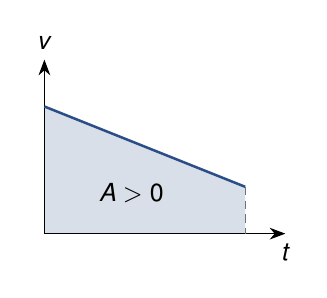
\begin{tikzpicture}[x=0.85cm,y=0.85cm]
\fill[bleu!18] (0,0)--(0,1.9)--(3.0,0.7)--(3.0,0) --cycle;
\node at (1.3,0.6) {\small$A>0$};
\draw[-{Stealth[length=2mm]}] (0,0)--(0,2.6) node[above]{\small$v$};
\draw[-{Stealth[length=2mm]}] (0,0)--(3.6,0) node[below]{\small$t$};
\draw[courbe] (0,1.9)--(3.0,0.7);
\draw[densely dashed,gris] (3.0,0.7)--(3.0,0);
\end{tikzpicture}

\small Sur $v(t)$ l'\textbf{aire} sous la courbe donne le \textbf{déplacement} : $\varDelta x = A$.\\
Si la courbe passe sous l'axe des temps, cette aire est \textbf{négative}.\\
Sur $v(t)$ la \textbf{pente} donne $a$.
\end{minipage}
\end{bloc}

\vspace{2mm}
\begin{bloc}{Où trouver quoi ?}
\small\renewcommand{\arraystretch}{1.25}
\begin{tabularx}{\linewidth}{@{}>{\bfseries\raggedright\arraybackslash}p{2.6cm}*{3}{>{\raggedright\arraybackslash}X}@{}}
Je cherche & \textbf{sur} $x(t)$ & \textbf{sur} $v(t)$ & \textbf{sur} $a(t)$\\\hline
Sens du mouvement & la courbe monte : sens de l'axe ; elle descend : sens opposé & $v>0$ : sens de l'axe ; $v<0$ : sens opposé & ---\\\hline
Vitesse & pente (corde : $v_{moy}$ ; tangente : $v$ instantanée) & lecture directe & ---\\\hline
Accélération & parabole ouverte vers le haut : $a>0$ ; vers le bas : $a<0$ & pente de $v(t)$ & lecture directe\\\hline
Déplacement $\boldsymbol{\varDelta x}$ & $x_2-x_1$ & aire sous $v(t)$ & ---\\\hline
Variation de vitesse $\boldsymbol{\varDelta v}$ & --- & $v_2-v_1$ & aire sous $a(t)$
\end{tabularx}
\end{bloc}

\vspace{2mm}
\begin{bloc}{Accélère ou décélère ?}
\begin{minipage}[t]{0.6\linewidth}
$v$ et $a$ de \textbf{même signe} $\Leftrightarrow$ $|v|$ augmente : le mobile \textbf{accélère}.

\smallskip
$v$ et $a$ de \textbf{signes opposés} $\Leftrightarrow$ $|v|$ diminue : le mobile \textbf{décélère}.
\end{minipage}\hfill
\begin{minipage}[t]{0.34\linewidth}\small
$v>0,\ a>0$ : accélère\\
$v<0,\ a<0$ : accélère\\
$v>0,\ a<0$ : décélère\\
$v<0,\ a>0$ : décélère
\end{minipage}

\smallskip
\small Attention : $a<0$ ne veut pas dire que le mobile ralentit. Compare toujours le signe de $a$ à celui de $v$.
\end{bloc}

\vspace{2mm}
\begin{bloc}{Problèmes numériques}
\begin{enumerate}[label=\textbf{\arabic*.},leftmargin=7mm,itemsep=2pt,topsep=2pt]
\item \textbf{Imaginer} la situation (faire un schéma).
\item \textbf{Choisir un repère} : origine O, sens de l'axe, instant $t=0$.
\item \textbf{Écrire les données} avec leur signe et des \textbf{unités cohérentes}.
\item \textbf{Identifier} le mouvement : MRU ou MRUA.
\item \textbf{Écrire les formules}.
\item \textbf{Résoudre} : équation du 1\textsuperscript{er} degré, du 2\textsuperscript{e} degré, ou système de deux équations à deux inconnues.
\item \textbf{Faire une phrase} de réponse.
\end{enumerate}
\end{bloc}

\end{document}
